% COMS 6998, Fall 2026 -- P3: Evaluation Plan & Initial Results
% Based on the course P3 template (coms6998-project-p3.zip) and the official ISCA 2026 IEEE class.
% Build: latexmk -pdf neural-symbolic-p3.tex  (or pdflatex, bibtex, pdflatex x2)
% Evidence: ../../PROGRESS.md and ../../results/p2/board/ (board_summary.json, raw CSVs).
% Figure data: python3 figures/generate-p3-figures.py (reads board_summary.json).
% Two pages excluding references; the reproduction appendix follows the references.

\documentclass[conference,10pt,letterpaper]{IEEEtran}
\usepackage[T1]{fontenc}
\usepackage{cite}
\usepackage{amsmath}
\usepackage{graphicx}
\usepackage{booktabs}
\usepackage{tabularx}
\IfFileExists{flushend.sty}{\usepackage{flushend}}{}% in the course template; not on every TeX install
\usepackage{xcolor}
\usepackage{tikz}
\usepackage{pgfplots}
\pgfplotsset{compat=1.16}
\usepackage[hyphens,obeyspaces]{url}
\usepackage[hidelinks]{hyperref}
\newcolumntype{Y}{>{\raggedright\arraybackslash}X}
\newcommand{\field}[1]{\textcolor{red!70!black}{\textit{[#1]}}}
% generated by generate-p3-figures.py from board_summary.json; do not edit
\newcommand{\WallFaithful}{3.88}
\newcommand{\WallLean}{2.99}
\newcommand{\WallDelta}{2.51}
\newcommand{\WallDeltaB}{2.49}
\newcommand{\WallRL}{2.50}
\newcommand{\WallRLB}{2.50}
\newcommand{\WallReplay}{1.40}


\title{ReasonLink: Characterizing and Optimizing the\\Handoff Between Neural and Symbolic Accelerators}
\author{\IEEEauthorblockN{Vayun Gupta (vg2684), Aaron Mano Cherian (amc2535)}
\IEEEauthorblockA{COMS 6998: AI-Native Computing $\mid$ Fall 2026\\
P3: Evaluation Plan \& Initial Results $\mid$ Due November 25, 2026, 11:59 PM ET}}

\begin{document}
\maketitle
\thispagestyle{plain}
\pagestyle{plain}

\section{Project Goal and Updates}
\textbf{Goal and claim.} When both stages of a neural--symbolic pipeline run on accelerators, does the handoff between them, converting neural outputs into solver input and moving it, become the bottleneck, and which interface mechanisms remove it? \textbf{Intended claim:} separating invariant constraints from per-input predictions, as compact solver-native updates plus solver state kept on chip, removes the handoff bottleneck. Overlap alone does not, and the extra value of generating the update in hardware depends on how fast the neural stage produces its outputs. We test \textbf{H1}: the full-image handoff is a large share of serial runtime, caused by rebuilding unchanged constraints rather than by the size of the neural output. We also test \textbf{H2}: double buffering hides only as much handoff as there is solve time to overlap.

\begin{figure*}[t]
\centering
% generated by generate-p3-figures.py from board_summary.json; do not edit
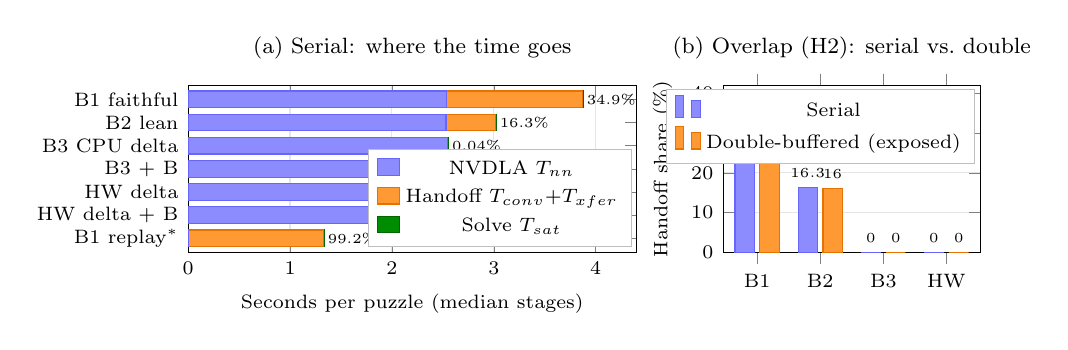
\begin{tikzpicture}
\begin{axis}[name=bd,width=0.60\textwidth,height=3.7cm,xbar stacked,bar width=6pt,
 xmin=0,xmax=4.4,ymin=-0.6,ymax=6.6,ytick={0,...,6},yticklabels={{B1 replay$^\ast$},{HW delta + B},{HW delta},{B3 + B},{B3 CPU delta},{B2 lean},{B1 faithful}},
 xlabel={Seconds per puzzle (median stages)},title={(a) Serial: where the time goes},
 tick label style={font=\scriptsize},label style={font=\scriptsize},title style={font=\footnotesize},
 xmajorgrids,grid style={gray!20},
 legend style={font=\scriptsize,at={(0.99,0.03)},anchor=south east,legend columns=1,draw=gray!50}]
\addplot[fill=blue!45,draw=blue!60] coordinates {(0.0002,0) (2.6155,1) (2.6185,2) (2.4587,3) (2.5478,4) (2.5305,5) (2.5378,6)};
\addplot[fill=orange!80,draw=orange!90!black] coordinates {(1.3277,0) (0.0001,1) (0.0001,2) (0.0005,3) (0.0005,4) (0.4848,5) (1.3310,6)};
\addplot[fill=green!55!black,draw=green!40!black] coordinates {(0.0110,0) (0.0030,1) (0.0101,2) (0.0031,3) (0.0102,4) (0.0106,5) (0.0110,6)};
\legend{NVDLA $T_{nn}$,Handoff $T_{conv}{+}T_{xfer}$,Solve $T_{sat}$}
\node[anchor=west,font=\tiny,inner sep=1pt] at (axis cs:1.3388,0) {99.2\%};
\node[anchor=west,font=\tiny,inner sep=1pt] at (axis cs:2.6185,1) {0.02\%};
\node[anchor=west,font=\tiny,inner sep=1pt] at (axis cs:2.6287,2) {0.02\%};
\node[anchor=west,font=\tiny,inner sep=1pt] at (axis cs:2.4623,3) {0.04\%};
\node[anchor=west,font=\tiny,inner sep=1pt] at (axis cs:2.5584,4) {0.04\%};
\node[anchor=west,font=\tiny,inner sep=1pt] at (axis cs:3.0260,5) {16.3\%};
\node[anchor=west,font=\tiny,inner sep=1pt] at (axis cs:3.8798,6) {34.9\%};
\end{axis}
\begin{axis}[at={(bd.east)},anchor=west,xshift=1.1cm,width=0.40\textwidth,height=3.7cm,
 ybar,bar width=7pt,ymin=0,ymax=42,symbolic x coords={B1,B2,B3,HW},xtick=data,
 ylabel={Handoff share (\%)},title={(b) Overlap (H2): serial vs.\ double},
 tick label style={font=\scriptsize},label style={font=\scriptsize},title style={font=\footnotesize},
 nodes near coords,nodes near coords style={font=\tiny},every node near coord/.append style={/pgf/number format/fixed,/pgf/number format/precision=1},
 ymajorgrids,grid style={gray!20},enlarge x limits=0.18,
 legend style={font=\scriptsize,at={(0.98,0.98)},anchor=north east,draw=gray!50}]
\addplot[fill=blue!45,draw=blue!60] coordinates {(B1,34.94) (B2,16.32) (B3,0.04) (HW,0.02)};
\addplot[fill=orange!80,draw=orange!90!black] coordinates {(B1,34.48) (B2,16.04) (B3,0.00) (HW,0.00)};
\legend{Serial,Double-buffered (exposed)}
\end{axis}
\end{tikzpicture}

\caption{Board results (VCU118; visual Sudoku puzzles 0--99; one run of 100 puzzles per configuration; stock NVDLA driver). (a)~Median per-puzzle stages, serial; labels give the median handoff share $(T_{conv}{+}T_{xfer})/T_{e2e}$. $^\ast$Replay substitutes recorded logits for NVDLA (diagnostic). HW-delta $T_{nn}$ includes per-cell push and credit waits and some SSH interference. (b)~Handoff share, serial vs.\ exposed share when double-buffered (a fully hidden solve, negative, is shown as 0). Quality is identical in every configuration: 81 SAT / 19 UNSAT; 100/100 answers equal the PySAT reference or are valid alternative grids.}
\label{fig:res}
\end{figure*}

\textbf{Updates since P2.} (1)~We dropped the third hypothesis (harder instances, crossover); the remaining time goes to the proposal's mechanisms and a clean evaluation. (2)~P2's board numbers were single runs, some disturbed by SSH monitoring (each login stalls the 78\,MHz CPU for 1--1.5\,s). The protocol now uses repeated, randomized runs with no network access during timing, and held-out puzzles (Table~\ref{tab:setup}). (3)~The neural stage is slower than it should be. NVDLA took 79\,ms per cell, about 99\% of an optimized run, for a LeNet of only about 2.3\,M multiply-accumulates. ESP builds NVDLA's kernel driver with \texttt{VERBOSE=1}, so its scheduler formats about 470 kernel-log messages per inference on the CPU (10 layers, 16 interrupt events), even with the console silenced. We built the driver with logging compiled out; measuring it is the first Milestone~4 run and motivates ablation A4. (4)~We received no written feedback on the midterm or P2; the changes above come from our own review of the P2 results.

\section{Evaluation Setup}
\textbf{Platform.} A VCU118 FPGA runs an ESP SoC~\cite{esp} (78\,MHz) with an Ariane CPU running Linux, NVDLA nv\_small~\cite{nvdla,espnvdla} in ESP's stock tile, and SAT-Accel~\cite{sataccel} in a third-party tile. We built SAT-Accel to RTL with Vitis HLS only, with our own shell and driver in place of v++ and XRT. ReasonLink's core lives in SAT-Accel's tile and reads NVDLA's logits from DRAM (Fig.~\ref{fig:pipe}). One bitstream runs every configuration. Stages are timed with \texttt{rdcycle}; SAT-Accel counts busy cycles, memory-stall cycles and DRAM reads.

\begin{figure}[t]
\centering
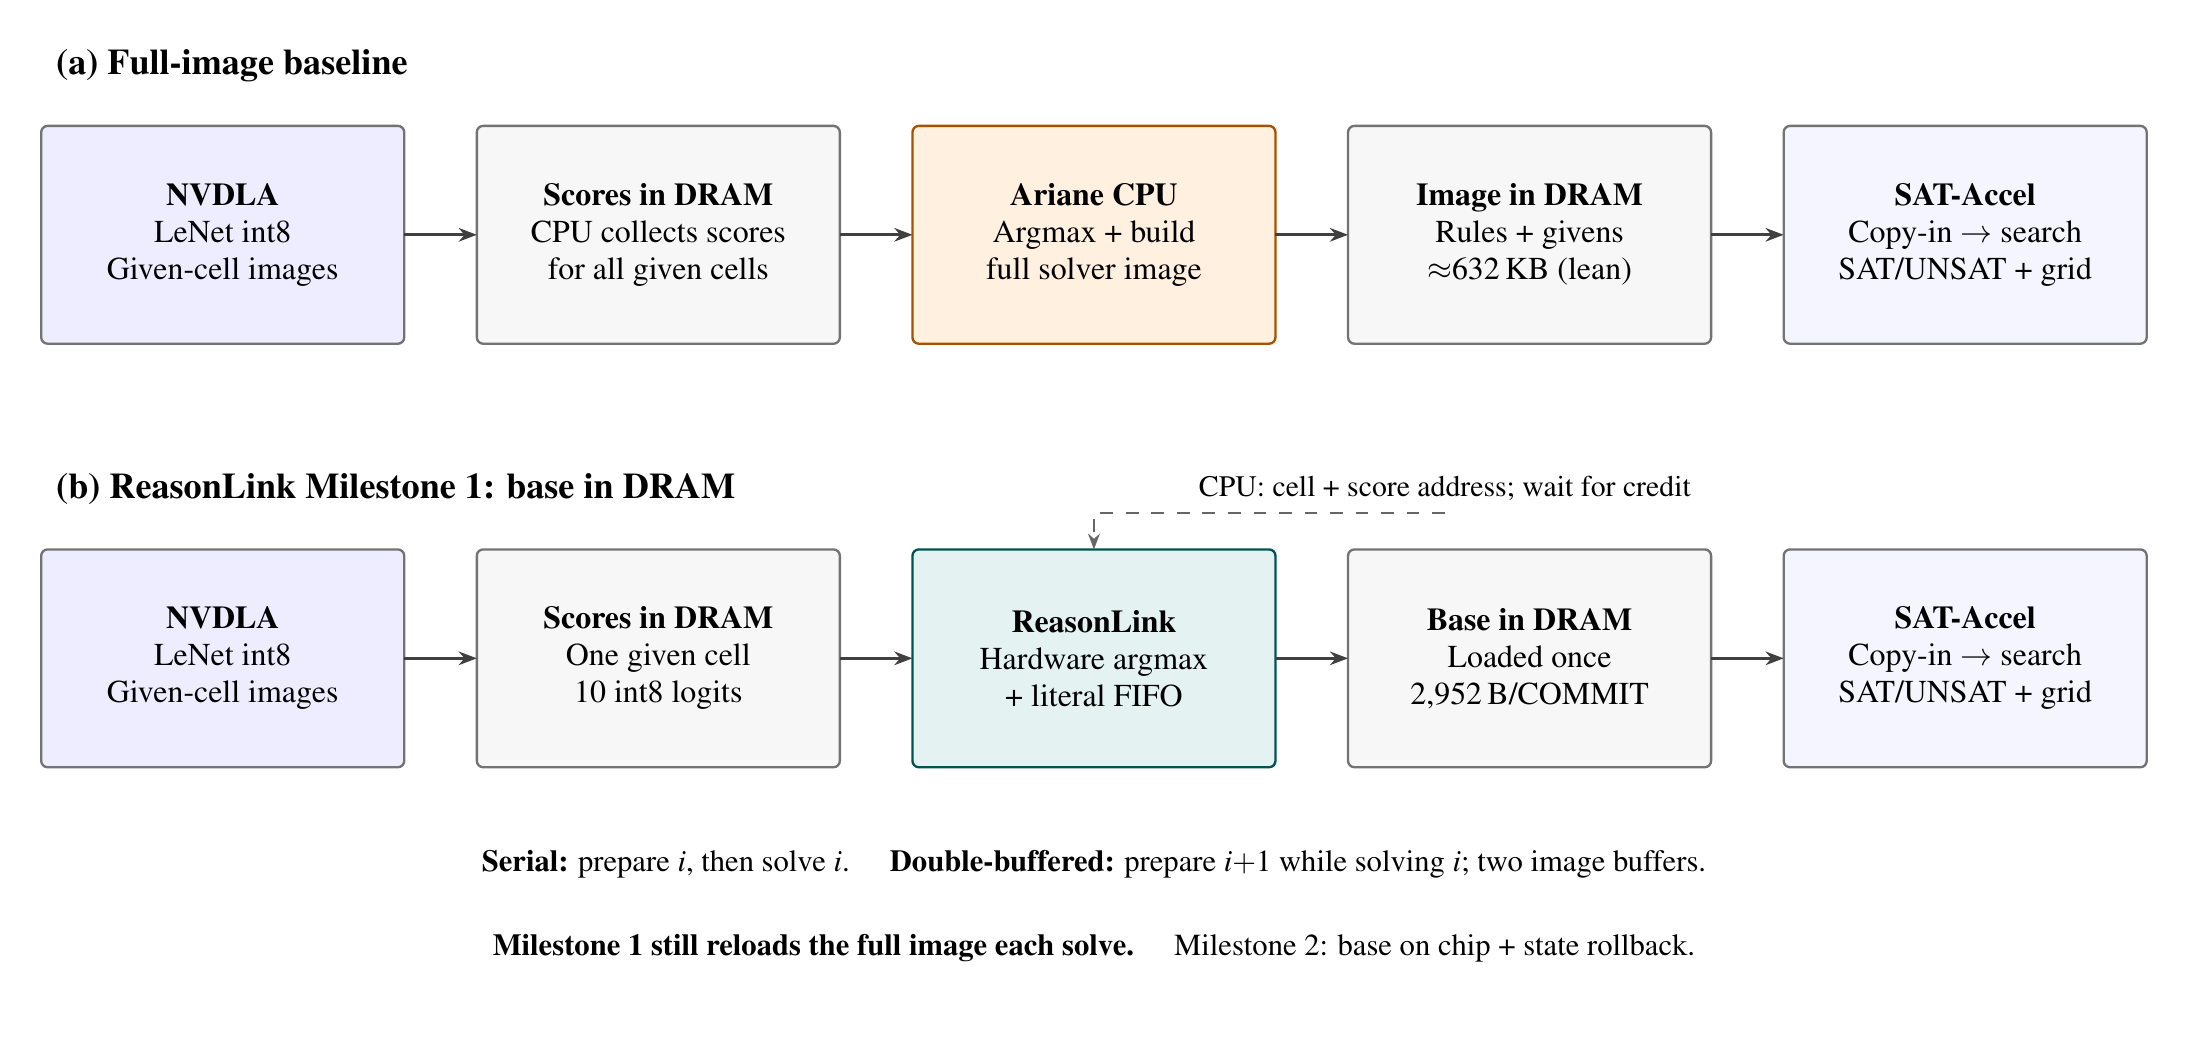
\includegraphics[width=\columnwidth]{figures/pipeline-diagram.png}
\caption{Handoff paths. (a)~Baselines: the CPU takes the argmax and rebuilds the full solver image for each puzzle. (b)~ReasonLink Milestone~1: hardware argmax into an on-chip literal FIFO, then a 2.9\,KB commit into a base image loaded once. Milestone~2 (+B) keeps the base formula on chip and restores only what a solve changes.}
\label{fig:pipe}
\end{figure}

\begin{table}[t]
\centering
\caption{Fixed evaluation setup.}
\label{tab:setup}
\footnotesize
\begin{tabularx}{\columnwidth}{@{}lY@{}}
\toprule
Workload & Visual Sudoku, 1,000 puzzles (24--40 givens, MNIST \emph{test} digits); one base CNF (729 vars, 11,988 clauses); givens become fixed decisions. Retrained int8 LeNet (99.2\%) on NVDLA. \\
Held-out & (a)~Puzzles 100--199, never run on the board (0--99 were used for debugging). (b)~SAT-Accel's 16 benchmark CNFs $\times$ 12 random decision sets for base reuse. \\
Baselines & \textbf{B1} faithful full image (SAT-Accel's host flow); \textbf{B2} lean full image (used regions only); \textbf{B3} CPU-generated delta (same compact update in software). Serial and double-buffered. \\
Ours & Hardware delta (ReasonLink); each delta path $\pm$ on-chip base reuse (+B). \\
Quality & SAT/UNSAT, grid, decisions equal to PySAT~\cite{pysat}; ground-truth accuracy; NVDLA vs.\ emulator digits. \\
Systems & Wall time per puzzle; medians of $T_{nn}, T_{conv}, T_{xfer}, T_{sync}, T_{sat}$; handoff share (exposed share if double-buffered); update bytes; SAT-Accel DRAM reads, stall share; LUT/URAM. \\
Protocol & 3 runs per configuration, random order, no SSH while timing; mean and min--max; hangs reported. Budget $\approx$6\,h board, one Linux rebuild, no new bitstream. \\
\bottomrule
\end{tabularx}
\end{table}

\section{Initial Results}
Fig.~\ref{fig:res} compares the baselines and ReasonLink on the board. All 13 configurations give identical SAT/UNSAT results (81/19; the UNSAT puzzles have a misread given), grids, and decision counts.

\textbf{H1 holds.} In B1, building the image takes 722\,ms and moving it 609\,ms against an 11\,ms solve: 34.9\% of the run, though NVDLA's output is only 310\,B of logits. B2 still spends 16.3\%. With NVDLA replaced by its recorded logits, the handoff is 99.2\% of B1's runtime. Both delta paths shrink the update from 5.3\,MB (B1) and 632\,KB (B2) to 3.9\,KB (CPU) or 2.9\,KB (ReasonLink), and the handoff to under 0.05\%. Base reuse then cuts the solve from 10.2 to 3.1\,ms and SAT-Accel's DRAM reads by 74\%. Wall time falls from \WallFaithful\,s (B1) and \WallLean\,s (B2) to \WallDelta\,s (B3) and \WallRL\,s (ReasonLink).
\textbf{H2 holds.} Double buffering leaves 34.5\% (B1) and 16.0\% (B2) exposed (Fig.~\ref{fig:res}b): it can hide at most the 11--13\,ms solve, while image building and NVDLA submission share one CPU.
\textbf{CPU and hardware deltas tie} (\WallDelta{} vs.\ \WallRL\,s; \WallDeltaB{} vs.\ \WallRLB\,s with +B). The core converts a cell in about 85 cycles, but the CPU's per-cell push and credit wait over ESP's APB bus (18\,$\mu$s per cell, 0.6\,ms per puzzle) cost more. Both are negligible next to 2.5\,s of NVDLA. Whether hardware generation helps thus depends on producer rate and per-cell control.

\section{Planned Ablations and Next Steps}
\begin{itemize}
\item \textbf{A1: delta placement, matched.} CPU vs.\ hardware delta, adding a CPU path that encodes each literal right after its cell is classified (ReasonLink's schedule) and one that writes the same 2,948\,B payload. This isolates where the delta is generated. \emph{Expected:} under 1\,ms difference while NVDLA dominates.
\item \textbf{A2: base reuse} ($\pm$B) on both delta paths, testing state reuse. \emph{Expected:} 60--70\% shorter solves, 74\% fewer DRAM reads; the cold first solve reported separately.
\item \textbf{A3: overlap,} serial vs.\ double for every handoff (H2). \emph{Expected:} helps only when the handoff is shorter than the stage it overlaps.
\item \textbf{A4: producer rate.} Stock driver, quiet driver, NVDLA writing to rotating output buffers (no per-cell credit wait), and logit replay. This tests when interface placement starts to matter. \emph{Expected:} B1/B2's handoff share rises toward 99\%; a CPU--hardware gap appears only at high rates.
\item \textbf{A5: queue depth and granularity.} ReasonLink queues up to 127 cells, so the CPU's push window $w\in\{1,4,16,81\}$ and per-cell vs.\ per-puzzle commits can be swept without a new bitstream. \emph{Expected:} wider windows amortize the per-cell control cost.
\end{itemize}

\textbf{Boundary case: stale state under base reuse.} Reuse is correct only if every on-chip change from the previous solve is undone. Without the literal-list tail cleanup, stale learned entries survive in 33/999 Sudoku and 62/176 benchmark runs. With it, the restored base matches a fresh copy-in byte for byte, and answers match in 1000/1000 and 192/192 runs. On the held-out benchmarks we will test cleanup disabled, a base that changes between solves (which must force a full copy-in), and heavy clause deletion (\texttt{hole7}, 16k conflicts). \textbf{Failure case:} NVDLA hung mid-task twice in P2 runs. The repeated runs log every hang, to show whether the quiet driver or the absence of SSH traffic changes the rate.

\textbf{Milestone 4 (Dec 7).} Measure the quiet driver. Add a puzzle-offset option for the held-out set. Rebuild the Linux image with the ReasonLink layout fix and the quiet driver. Run all 13 configurations three times, then A1, A2, A4 and the boundary study. \textbf{Main risk:} if NVDLA stays bound by its runtime after the driver fix, the CPU--hardware comparison stays a tie. We would report that as a negative result explained by per-cell control cost.

\smallskip\noindent\textbf{AI use.} We used Claude (Anthropic) to help write analysis and board scripts and to draft this report. Every number traces to our board logs, simulation outputs, or the repository's result files.

\bibliographystyle{IEEEtran}
\bibliography{neural-symbolic-references,p1-additional-references}

\appendices
\section{Reproduction}
{\footnotesize
From the repository root unless noted. Board steps run on the ESP server after \path{source ~/esp/socs/reasonlink-vcu118/fpga-script.sh} (lab FPGA settings; the scripts also source it); the board's root password is passed as \texttt{RL\_PW} and never stored.
\begin{enumerate}
\item Fig.~\ref{fig:res} data: \path{cd "Project Updates/P3 Evaluation Plan"; python3 figures/generate-p3-figures.py} (reads \path{results/p2/board/csv/board_summary.json}).
\item Board summary from the raw CSVs: \path{python3 board/summarize_board.py results/p2/board/csv}.
\item Board state of the P2 runs, no rebuild: \path{RL_PW=... RL_BACKUP=~/m2/backup_reasonlink_20261105 ~/m2/boot_and_run.sh <batch>}.
\item Quiet NVDLA driver: copy \path{~/esp/accelerators/third-party/NV_NVDLA/sw/kmd} to \path{~/m2/nvdla_quiet/}; in its \path{kmd/}: \path{make KDIR=~/esp/socs/reasonlink-vcu118/soft-build/ariane/linux-build ARCH=riscv CROSS_COMPILE=riscv64-unknown-linux-gnu- VERBOSE=0}.
\item Driver profile (first M4 run): \path{RL_PW=... ~/m2/nvprof_run.sh}, then \path{python3 board/nvprof_summary.py <fetched CSVs> results/p2/board/csv}.
\end{enumerate}}
\end{document}
